\documentclass[11pt]{article}
\usepackage[nohead,margin=1.50in]{geometry} %set margins
\usepackage{amsmath,amssymb,amsthm,pdiag,amscd,epic} %packages
\usepackage{graphicx}  
\usepackage{enumitem}
 \setlist{topsep=1pt,itemsep=0pt,parsep=1pt,leftmargin=0.7cm}
 \setenumerate[1]{label=(\alph*)}

\newenvironment{problems}
{\begin{enumerate}[topsep=1pt,itemsep=0pt,parsep=2pt,leftmargin=0.6cm,%
 label={\arabic*.}, ref=\arabic*]\small%
}
{
 \end{enumerate}
}

%%% Define some theorem and example environments. The starred versions
%%% are un-numbered and the unstarred versions are numbered.
\newtheoremstyle{plain}
  {\topsep}   % ABOVESPACE
  {\topsep}   % BELOWSPACE
  {\slshape}  % BODYFONT
  {0pt}       % INDENT (empty value is the same as 0pt)
  {\bfseries} % HEADFONT
  {.}         % HEADPUNCT
  {5pt plus 1pt minus 1pt} % HEADSPACE
  {}          % CUSTOM-HEAD-SPEC

\swapnumbers
\newtheorem{thm}{Theorem}[section]
\newtheorem{lem}[thm]{Lemma}
\newtheorem{prop}[thm]{Proposition}
\newtheorem{cor}[thm]{Corollary}
\newtheorem*{thm*}{Theorem}
\newtheorem*{lem*}{Lemma}
\newtheorem*{prop*}{Proposition}
\newtheorem*{cor*}{Corollary}

\theoremstyle{definition}
\newtheorem{defn}[thm]{Definition}
\newtheorem{example}[thm]{Example}
\newtheorem{examples}[thm]{Examples}
\newtheorem{rmk}[thm]{Remark}
\newtheorem{conv}[thm]{Convention}
\newtheorem*{defn*}{Definition}
\newtheorem*{example*}{Example}
\newtheorem*{examples*}{Examples}
\newtheorem*{rmk*}{Remark}
\newtheorem*{conv*}{Convention}

%%% Define some convenient abbreviations for common mathematical
%%% notations.
\newcommand{\R}{\mathbb{R}} % use \R for the real numbers
\newcommand{\C}{\mathbb{C}} % use \C for the complex numbers
\newcommand{\Z}{\mathbb{Z}} % use \Z for the integers
\newcommand{\Q}{\mathbb{Q}} % use \Q for the rationals
\newcommand{\N}{\mathbb{N}} % use \N for the natural numbers
\newcommand{\compose}{\circ} % functional composition
\renewcommand{\implies}{\Rightarrow}
\renewcommand{\iff}{\Leftrightarrow}
\newcommand{\F}{{\mathbb F}}
\newcommand{\gen}[1]{\langle #1 \rangle}
\newcommand{\End}{\operatorname{End}}
\newcommand{\GL}{\mathrm{GL}}
\newcommand{\SL}{\mathrm{SL}}
\renewcommand{\O}{\mathrm{O}}
\newcommand{\SO}{\mathrm{SO}}
\newcommand{\U}{\mathrm{U}}
\newcommand{\SU}{\mathrm{SU}}
\newcommand{\g}{\mathfrak{g}}
\newcommand{\transpose}{\mathsf{T}}
\newcommand{\B}{\mathcal{B}}
\newcommand{\Rep}{\operatorname{Rep}}
\newcommand{\Mat}{\operatorname{Mat}}
\newcommand{\inner}[2]{\langle #1, #2 \rangle}
\newcommand{\sgn}{\operatorname{sgn}}
\newcommand{\n}{\underline{\mathbf{n}}}
\newcommand{\Sym}{\mathbb{S}}
\newcommand{\Alt}{\mathbb{A}}
\newenvironment{perm}[2]{\left(\begin{smallmatrix}#1 \\ #2}{\end{smallmatrix}\right)}
\newcommand{\Map}{\operatorname{Map}}
\newcommand{\Rot}{\Theta}
\newcommand{\D}{\mathbb{D}}


\allowdisplaybreaks
\parskip=2pt

%\title{Document Title}
%\author{author's name}

\begin{document}%\maketitle
\setcounter{section}{8}



\section{Symmetry groups}\index{symmetry~group}\noindent
What are groups good for, anyway? One answer is that they can be used
to quantify \emph{symmetry}.  Measuring symmetry is what groups
do. Symmetry is ubiquitous in nature, and is an important component of
art and music. In chemistry, symmetry groups distinguish between
different molecular structures and describe properties of crystals; in
physics, symmetry groups help us understand interactions of subatomic
particles. The symmetry group of the Rubik's cube is helpful for
solving the puzzle. The original application of symmetry groups was in
the theory of polynomial equations, where Galois showed that the
symmetry group of the equation determines whether or not it can be
solved in terms of radicals. We will only touch on a few simple
examples of symmetry groups. This is a complex topic, which can be
studied from several different viewpoints.




\begin{example}[rotation group of a square]\index{rotation group} 
\label{exmpl:square}%
A \emph{rotational symmetry} of a square is a rotation of the square
which brings it back to itself; it is always assumed that such
rotations fix the center point of the square. If the square has no
marks, we would not be able to tell whether or not it was
rotated. Such rotations are said to \emph{preserve} the square.

The \emph{rotation group} of the square is the set of all of its
rotational symmetries. This set is a group, because we can compose
rotations by following one by another. 

How many rotational symmetries (of the square) are there? The answer
is that it depends on how we decide to count them. It is useful to
number the vertices of the square in order to keep track of the effect
of rotations. Let's number the vertices as follows:
\[
\begin{minipage}{20mm}
  \setlength{\unitlength}{0.4mm}
\begin{picture}(25,25)(0,0)
\thicklines \tiny
\drawline[40](0,0)(20,0)
\drawline[40](20,0)(20,20)
\drawline[40](20,20)(0,20)
\drawline[40](0,20)(0,0)

\put(22,22){\makebox(0,0){1}}
\put(-2,22){\makebox(0,0){2}}
\put(-2,-2){\makebox(0,0){3}}
\put(22,-2){\makebox(0,0){4}}
\end{picture}
\end{minipage}
\]
\par\smallskip\noindent 
We will call this configuration the \emph{start} configuration. Let
$i$ be the rotation by zero degrees. This rotation does nothing to the
configuration, so $i$ is the identity rotation. Another rotational
symmetry is the counterclockwise rotation $r$ by 90 degrees
(i.e.\ $\pi/2$ radians), depicted below:
\[
\begin{CD}
\begin{minipage}{20mm}
  \setlength{\unitlength}{0.4mm}
\begin{picture}(22,22)(0,0)
\thicklines \tiny
\drawline[40](0,0)(20,0)
\drawline[40](20,0)(20,20)
\drawline[40](20,20)(0,20)
\drawline[40](0,20)(0,0)

\put(22,22){\makebox(0,0){1}}
\put(-2,22){\makebox(0,0){2}}
\put(-2,-2){\makebox(0,0){3}}
\put(22,-2){\makebox(0,0){4}}
\end{picture}
\end{minipage} 
@>r>> \qquad
\begin{minipage}{20mm}
  \setlength{\unitlength}{0.4mm}
\begin{picture}(22,22)(0,0)
\thicklines \tiny
\drawline[40](0,0)(20,0)
\drawline[40](20,0)(20,20)
\drawline[40](20,20)(0,20)
\drawline[40](0,20)(0,0)

\put(22,22){\makebox(0,0){4}}
\put(-2,22){\makebox(0,0){1}}
\put(-2,-2){\makebox(0,0){2}}
\put(22,-2){\makebox(0,0){3}}
\end{picture}
\end{minipage}
\end{CD}
\]
\par\smallskip\noindent The rotation $r$ actually does something to
the square, so it is not the same as the identity $i$.  The rotations
$r^2 =$ rotation by 180 degrees, and $r^3 =$ rotation by 270 degrees
are also symmetries of the square.  Let's adopt the convention that
two symmetries are consider the same if and only if they are
indistinguishable from one another in terms of the numbering of the
vertices. Then $r^4 =$ rotation by 360 degrees will bring the square
back to its starting position, so $r^4 = i$. 

We have found four distinct rotational symmetries thus far: namely the
rotations $i, r, r^2, r^3$, so the rotation group of the square
contains at least the elements $\{i, r, r^2, r^3\}$. Are there any more
rotational symmetries? The answer is no. It is true that $r^{-1} =$
rotation by $-90$ degrees is a symmetry, but it is the same as the
rotation by $270$ degree; i.e., $r^{-1} = r^3$. So $r^{-1}$ is already
counted. Similarly, you may think that $r^5 = $ rotation by 450
degrees is a new rotation, but since $r^4=i$ it follows that $r^5 =
r$. So $r^5$ is not anything new. It turns out that any rotational
symmetry you might think of is already in our list. So the rotation
group of a square is the group
\[
  G = \{i, r, r^2, r^3 \} = \gen{r}
\]
of order $4$, generated by the basic rotation $r$. 
\end{example}



\begin{example}[improper symmetries]\index{improper symmetry}
There are other symmetries of a square besides the rotations.  Let
$h$ be the reflection of the points on the square across its
horizontal axis. The effect of $h$ can be depicted as follows:
\[
\begin{CD}
\begin{minipage}{20mm}
  \setlength{\unitlength}{0.4mm}
\begin{picture}(22,22)(0,0)
\thicklines \tiny
\drawline[40](0,0)(20,0)
\drawline[40](20,0)(20,20)
\drawline[40](20,20)(0,20)
\drawline[40](0,20)(0,0)

\put(22,22){\makebox(0,0){1}}
\put(-2,22){\makebox(0,0){2}}
\put(-2,-2){\makebox(0,0){3}}
\put(22,-2){\makebox(0,0){4}}
\end{picture}
\end{minipage} 
@>h>> \qquad
\begin{minipage}{20mm}
  \setlength{\unitlength}{0.4mm}
\begin{picture}(22,22)(0,0)
\thicklines \tiny
\drawline[40](0,0)(20,0)
\drawline[40](20,0)(20,20)
\drawline[40](20,20)(0,20)
\drawline[40](0,20)(0,0)

\put(22,22){\makebox(0,0){4}}
\put(-2,22){\makebox(0,0){3}}
\put(-2,-2){\makebox(0,0){2}}
\put(22,-2){\makebox(0,0){1}}
\end{picture}
\end{minipage}
\end{CD}
\]
\par\smallskip\noindent
Reflections are sometimes called \emph{improper} symmetries; in this
parlance the rotations would be called \emph{proper} symmetries. 

Are there any other improper symmetries of the square? Yes. There
are three other reflections: 

$v=$ reflection across the vertical axis, 

$d_1=$ reflection across the diagonal line connecting vertices 1 and 3, 

$d_2=$ reflection across the diagonal line connecting vertices 2 and 4.

\noindent
It turns out that we have found them all. There are precisely four
improper symmetries of the square, namely $\{ h, v, d_1, d_2 \}$.

The improper symmetries do \emph{not} form a group, however. To be a
group, a set must be closed under products and inverses, and the set
$\{ h, v, d_1, d_2 \}$ of improper symmetries is not closed under
products, because the square of a reflection is the identity $i$ and
$i$ is not in the set.

However, if we combine the proper and improper symmetries in a set, we
do obtain a group. So the set $\D_4 = \{ i,r,r^2,r^3, h, v, d_1, d_2
\}$ of proper and improper symmetries of the square is a group; it is
called the \emph{symmetry group} of the square. One nice way to see
that it really is a group is to work out its multiplication table.

As already mentioned, we multiply symmetries by composition, i.e.,
following one by the other. For example, to compute the product $hr$
means to first do $r$ and then do $h$. (Recall that $hr = h \compose
r$ means $r$ followed by $h$.)  The product $hr$ can be depicted by:
\[
\begin{CD}
\begin{minipage}{20mm}
  \setlength{\unitlength}{0.4mm}
\begin{picture}(22,22)(0,0)
\thicklines \tiny
\drawline[40](0,0)(20,0)
\drawline[40](20,0)(20,20)
\drawline[40](20,20)(0,20)
\drawline[40](0,20)(0,0)

\put(22,22){\makebox(0,0){1}}
\put(-2,22){\makebox(0,0){2}}
\put(-2,-2){\makebox(0,0){3}}
\put(22,-2){\makebox(0,0){4}}
\end{picture}
\end{minipage} 
@>r>> \qquad
\begin{minipage}{20mm}
  \setlength{\unitlength}{0.4mm}
\begin{picture}(22,22)(0,0)
\thicklines \tiny
\drawline[40](0,0)(20,0)
\drawline[40](20,0)(20,20)
\drawline[40](20,20)(0,20)
\drawline[40](0,20)(0,0)

\put(22,22){\makebox(0,0){4}}
\put(-2,22){\makebox(0,0){1}}
\put(-2,-2){\makebox(0,0){2}}
\put(22,-2){\makebox(0,0){3}}
\end{picture}
\end{minipage}
@>h>> \qquad
\begin{minipage}{20mm}
  \setlength{\unitlength}{0.4mm}
\begin{picture}(22,22)(0,0)
\thicklines \tiny 
\drawline[40](0,0)(20,0)
\drawline[40](20,0)(20,20)
\drawline[40](20,20)(0,20)
\drawline[40](0,20)(0,0)

\put(22,22){\makebox(0,0){3}}
\put(-2,22){\makebox(0,0){2}}
\put(-2,-2){\makebox(0,0){1}}
\put(22,-2){\makebox(0,0){4}}
\end{picture}
\end{minipage}
\end{CD}
\]
\par\smallskip\noindent The net result of combining the two operations
in succession is the same as the reflection $d_2$,
\[
\begin{CD}
\begin{minipage}{20mm}
  \setlength{\unitlength}{0.4mm}
\begin{picture}(22,22)(0,0)
\thicklines \tiny
\drawline[40](0,0)(20,0)
\drawline[40](20,0)(20,20)
\drawline[40](20,20)(0,20)
\drawline[40](0,20)(0,0)

\put(22,22){\makebox(0,0){1}}
\put(-2,22){\makebox(0,0){2}}
\put(-2,-2){\makebox(0,0){3}}
\put(22,-2){\makebox(0,0){4}}
\end{picture}
\end{minipage} 
@>d_2>> \qquad
\begin{minipage}{20mm}
  \setlength{\unitlength}{0.4mm}
\begin{picture}(22,22)(0,0)
\thicklines \tiny
\drawline[40](0,0)(20,0)
\drawline[40](20,0)(20,20)
\drawline[40](20,20)(0,20)
\drawline[40](0,20)(0,0)

\put(22,22){\makebox(0,0){3}}
\put(-2,22){\makebox(0,0){2}}
\put(-2,-2){\makebox(0,0){1}}
\put(22,-2){\makebox(0,0){4}}
\end{picture}
\end{minipage}
\end{CD}
\]
\par\smallskip\noindent so we write $hr = d_2$. By doing similar
calculations, one can work out the full multiplication table of the
symmetry group $\D_4$. This group is called a \emph{dihedral group}.
\end{example}

\begin{rmk}
  Improper symmetries can also be viewed as rotations. The reflection
  of a plane figure in a given line may be regarded as a rotation of
  the plane containing the figure by $\pi$ radians about that line,
  which serves as the axis of the rotation. For this it is necessary
  to work in three dimensions. The proper rotations, on the other
  hand, are rotations of the plane containing the figure. Proper
  rotations take place entirely in the plane, and thus do not require
  three dimensions to describe.
\end{rmk}


The following terminology, which is a basic concept, will be used
frequently.


\begin{defn}\index{isomorphism}
  Let $G,H$ be groups. An \emph{isomorphism} from $G$ onto $H$ is a
  bijection $f: G \to H$ which preserves products (in the sense that
  $f(ab) = f(a)f(b)$ for all $a,b \in G$). We say that $G$ is
  \emph{isomorphic to} $H$ (written as $G \cong H$) if there is an
  isomorphism $f: G \to H$. 
\end{defn}

The fact that an isomorphism is a bijection means that if $G \cong H$
then $|G|=|H|$. The fact that it preserves products means that the
multiplication tables for the two groups are identical, except for the
names of the elements. Of course, names are purely arbitrary labels
and have no intrinsic meaning, so it follows that isomorphic groups
are essentially the ``same'' group apart from the names of the
elements. So, informally speaking, the word ``isomorphic'' means ``the
same structure.''

The concept of isomorphism may be initially somewhat abstract, so let's
look at a concrete example. 
 

\begin{example}
Let $G$ be the symmetry group of the square, as in the previous
example.  We can think of each symmetry in $G$ as corresponding to the
permutation whose second row records the {\em position} in which each
vertex ends up under the motion. In short, we say that each symmetry
in $G$ can be \emph{represented} by a permutation. The representation
is given in the following table.
\[
\begin{array}{|cc|} \hline 
  \text{symmetry} & \text{permutation} \\ \hline 
  i & (1)\\
  r & (1,2,3,4)\\
  r^2 & (1,3)(2,4)\\
  r^3 & (4,3,2,1)\\
  h & (1,4)(2,3)\\
  v & (1,2)(3,4)\\
  d_1 & (2,4)\\
  d_2 & (1,3)\\ \hline
\end{array}
\]
Note that the permutations are written in terms of the cycle notation.
A bit of thought reveals that the 8 permutations in the rightmost
column of the table form a permutation group $P$. The function $f:
\D_4 \to P$ which sends the element in the left column to the
corresponding permutation in the right column defines a bijection from
$\D_4$ onto $P$. Although it is tedious do do so at this point, it can
be checked that $f$ preserves products. Thus $f$ is an isomorphism and
$\D_4 \cong P$. So we may think of $\D_4$ as a permutation group if we
so desire.

Furthermore, if we restrict the isomorphism $f$ to the group $G$ of
proper symmetries (the rotation group) of the square, then we obtain
an isomorphism of $G$ onto the permutation group $H = \gen{\alpha}$,
where $\alpha = (1,2,3,4)$. The group $H = \{ id, \alpha, \alpha^2,
\alpha^3 \}$ is a cyclic group of order 4, so we have proved that the
group $G$ of proper symmetries of a square is isomorphic to a cyclic
group of order 4.
\end{example}






\begin{example}\label{ex:dihedral}[symmetry group of the regular $n$-gon]
Fix a regular $n$-sided polygon, where $n \ge 3$. The group of all
symmetries of the polygon is denoted by $\D_n$\index{D@$\D_n$}; it is
known as the {\em dihedral group}\index{dihedral group} of order
$2n$. When $n=4$ this is the symmetry group $\D_4$ of a square.

Clearly, $r=$ rotation by $2\pi/n$ radians preserves the 
polygon. Then $r^k =$ rotation by $2k\pi/n$ radians, and it preserves
the polygon as well. Notice that $r^n = i$, the identity.
So the proper symmetry group (the rotation group) of the polygon is
\[
  G = \{ i, r, r^2, \dots, r^{n-1 }\} = \gen{r}.
\]
We have $|G| = n$, so there are $n$ proper symmetries. 

There are also $n$ improper symmetries, the reflections. Let $\ell$ be
a line which bisects the polygon (so that the two parts on opposite
sides of $\ell$ are congruent). Then reflection across the line $\ell$
is an improper symmetry. Let $d = $ the reflection that sends
vertex $n$ to itself. Then with a bit of work it is possible to show
that the set 
\[
  \{d, dr, \dots, d r^{n-1}\}
\]
is the set of improper symmetries of the polygon. This is due to the
fact that following a rotation by a reflection always produces another
reflection, and all reflections are produced this way.  So the
dihedral group $\D_n$ is the group
\[
  \D_n = \{ i, r, r^2, \dots, r^{n-1}, d, dr, dr^2, \dots, d r^{n-1}
  \}.
\]
The dihedral group consists of $n$ rotations and $n$ reflections, for
a total of $2n$ symmetries. Thus $|\D_n| = 2n$. 

With a bit of effort one can check that the generating rotation $r$
and the reflection $d$ are related by the nice formula $$r d r = d$$
which is equivalent to the relations $rd = d r^{-1} = d
r^{n-1}$. These relations are all one needs to compute products of
elements of $\D_n$.
\end{example}



\section*{Exercises}
\begin{problems}

\item \label{prob:tri} Cut a piece of paper in the shape of an
equilateral triangle and number its vertices (on both sides) in order
counterclockwise, as shown in the figure below:
\[
\begin{minipage}{20mm}
  \setlength{\unitlength}{0.7mm}
\begin{picture}(25,20)(0,0)
\thicklines \tiny
\drawline[40](0,0)(20,0)
\drawline[40](0,0)(10,17.32)
\drawline[40](10,17.32)(20,0)

\put(10,20){\makebox(0,0){2}}
\put(-2,-2){\makebox(0,0){3}}
\put(22,-2){\makebox(0,0){1}}
\end{picture}
\end{minipage}
\]
Let $r=$ rotation counterclockwise by $2\pi/3$ radians; note that
$r^3 = i$ is the identity rotation. Let $d_j = $ reflection in the
bisector which fixes the point $j$, for $j=1, 2, 3$.  Then the
symmetries of the triangle are $\D_3 = \{i, r, r^2, d_1, d_2, d_3\}$.
Using these labels, work out the multiplication table for the symmetry
group $\D_3$.

\item Cut a piece of paper into an isosceles triangle which is not
  equilateral. Describe its symmetry group $G$, and compute its
  multiplication table. 

\item In biology, it is pointed out that many animals have
  \emph{bilateral symmetry}. Humans are an example. The human body has
  bilateral symmetry (if the arms and legs are in a symmetric
  position). What is the symmetry group of the human form? How does it
  relate to the group $G$ of the previous problem?


\item Cut a square piece of paper and number the vertices (on both
  sides) as in Example \ref{exmpl:square}. Using this tool, make a
  multiplication table for the group $\D_4$.

\item Cut a rectangular piece of paper that is \emph{not} square and
  number the vertices. Using this tool, find the symmetry group of the
  non-square rectangle. Give the order and a multiplication table of
  this group. 

\item How much symmetry does a word have? Let's define a \emph{word}
  in an alphabet $A$ to be any finite string of symbols from $A$. For
  instance, if $A = \{a,b\}$ then $w_1=abba$, $w_2=baba$, $w_3=aba$,
  and $w_4 = bbb$ are all words over $A$. Let's define a
  \emph{symmetry} of a word $w$ to be any permutation of the word $w$
  which preserves the word. For instance, the transposition $(1,3)$,
  which interchanges the letters in positions 1 and 3, preserves the
  words $w_2, w_3$ but not $w_1$. Let $G(w)$ be the group of all
  symmetries of a word $w$.
  \begin{enumerate}
  \item Compute $G(w)$ for $w = w_1, w_2, w_3, w_4$ as above.
  \item Which of these four words has the \emph{most} symmetry?
  \end{enumerate}

  

\item 
  \begin{enumerate}
  \item Prove that $rhr = h$ in $\D_4$ by giving a geometric argument.
  \item Similarly, prove that $rd_2r = d_2$ in $\D_4$.
  \end{enumerate}

\item Given the fact that
  $\D_5 = \{ i,r,r^2,r^3,r^4, d, dr, dr^2, dr^3, dr^4 \}$, where $r,d$
  are as defined in Example \ref{ex:dihedral}, compute its
  multiplication table. Every product in your table must be an element
  of $\D_5$.

\item Use the equation $rdr = d$ from Example \ref{ex:dihedral} to
  prove that in $\D_n$ we have $r^kd = d r^{n-k}$ for $k = 1, 2, \dots,
  n-1$. 


\item Make a table of the permutation representation of
  $\D_3 = \{i, r, r^2, d_1, d_2, d_3\}$, using the labels introduced
  in Problem \ref{prob:tri}. Use the table to show that
  $\D_3 \cong \Sym_3$. Explain how your isomorphism is defined.
  
\item Is $\D_4 \cong \Sym_4$? Justify your answer.


\item 
  \begin{enumerate}
  \item Find the permutations representing $r,d \in \D_n$, as defined
    in Example \ref{ex:dihedral}.
  \item Then describe a permutation group which is isomorphic to
    $\D_n$.
  \item Use the isomorphism from part (b) to show that $rdr = d$.
  \end{enumerate}

\end{problems}


\newpage
\section{The Platonic solids}\index{Platonic solids}
Now we turn our attention to symmetry groups in 3-dimensional
euclidean geometry. First, we consider the classification of regular
polyhedra in solid geometry.

Plane geometry is the study of figures in the plane $\R^2$, while
solid geometry means the study of solid figures in $\R^3$ (three
dimensions instead of two). A {\em platonic solid} is a regular figure
in three dimensions which is analogous to the regular $n$-gons in two
dimensions.  While in two dimensions we have infinitely many such
figures (the regular $n$-gon for each $n$) in three dimensions
\emph{there are only five regular solids}. 

We will assume this, as the proof would take too much of our time, but
if you want to know more, there is an excellent Wikipedia article on
this topic that not only delves into the history but also explains
several proofs. The classification of regular solid polyhedra is the
final result in Euclid's {\em Elements}; this was the first published
proof.

%\begin{figure} [ht]
       \begin{center}
       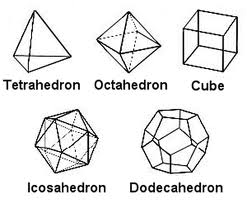
\includegraphics{platonic.jpg}
       \end{center}
       %\caption{The Platonic Solids}
       %\label{fig1}
%\end{figure}

Here are the names of the five platonic solids, which are pictured
above.  The {\em tetrahedron} is a $4$-sided solid with equilateral
triangles as faces; the {\em cube} is a $6$-sided solid with square
faces; the {\em octahedron} is an $8$-sided solid with equilateral
triangles as faces; the {\em dodecahedron} is a $12$-sided solid with
faces which are regular pentagons; and finally the {\em icosahedron}
is a $20$-sided solid with equilateral triangles for its faces.
 


\begin{example}[proper symmetry groups of the Platonic solids]
Let us begin by describing the {\em proper} symmetries (the rotations)
of the five Platonic solids. It is already a difficult problem to
count them in some effective way.

The proper symmetry group of the tetrahedron is the {\em tetrahedral
  group}\index{tetrahedral group}, denoted by $\mathbf{T}$.  It turns
out that $\mathbf{T} \cong \Alt_4$. This can be demonstrated by
considering a permutation representation of the tetrahedron. One can
number the vertices and write out the permutations corresponding to
the rotations, it turns out that these are precisely the elements of
$\Alt_4$. The details are tedious.  The isomorphism $\mathbf{T} \cong
\Alt_4$ means in particular that $|\mathbf{T}| = |\Alt_4| = 12$. So
there are 12 proper rotations of a tetrahedron.

The proper symmetries of the cube give us another group, called the
{\em octahedral group}\index{octahedral group}, and written as
$\mathbf{O}$. We have $|\mathbf{O}| = 24$.

The proper symmetries of the octahedron give us a group isomorphic
with $\mathbf{O}$, so we don't get a new group from this solid. 

This is due to the fact that the cube and the octahedron are {\em
  dual} to one another. To obtain the dual of a regular polyhedron,
put a dot in the center of each face, and let the dots be the vertices
of a new polyhedron.  This new polyhedron is the dual of the original
one. It is not hard to see that the symmetry group of a polyhedron
must be the same as the symmetry group of its dual.

The proper symmetries of the dodecahedron give us a third symmetry
group, called the {\em icosahedral group}\index{icosahedral group},
and denoted by the symbol $\mathbf{I}$. This group has $60$ elements;
in fact it is isomorphic with the alternating group $\Alt_5$.  The
proper symmetries of the icosahedron give us a group isomorphic with
$\mathbf{I}$, so we don't get a new group from this solid. This is due
to the fact that the icosahedron is the dual of the dodecahedron.


Summary: The proper symmetries of the five Platonic solids give us
just three new symmetry groups: $\mathbf{T}\cong \Alt_4$;
$\mathbf{O}$; and $\mathbf{I}\cong \Alt_5$. Two of them are isomorphic
to groups we have seen before, but the octahedral group $\mathbf{O}$
is new.
\end{example}


\begin{example}[improper symmetries of the Platonic solids]
\index{improper symmetry}%
As in the case of regular polygons, it turns out that there are
improper symmetries of all of the regular polyhedra. They are a bit
harder to describe, but it turns out that there are always as many
improper symmetries as there are proper ones, just as in the polygon
case.

When we include the improper symmetries, we get the full symmetry
group. The full symmetry group of each Platonic solid therefor has
twice as many elements as its proper symmetry group. We need to
develop more theory in order to say more about this topic, so we leave
this for now.
\end{example}





\section*{Exercises}
\begin{problems}

\item Explain why two finite groups of different cardinality cannot
  be isomorphic.

\item Prove that the proper symmetry group of the tetrahedron is
  isomorphic to the alternating group $\Alt_4$. One way to do this is
  via a permutation representation. (Number the vertices of the
  tetrahedron and regard symmetries as permutations of the vertices.)

\item Using the same idea as in the previous problem, prove that the
  full symmetry group of the tetrahedron is the symmetric group
  $\Sym_4$.

\item Explain why the symmetry group of a regular solid must be the
  same as that of its dual.

\item Describe the 24 proper symmetries of the cube in words. 

\end{problems}
\end{document}








%%%%%%%%%%%%%%%%%%%%%%%%%%%%%%% exercises %%%%%%%%%%%%%%%%%%
\item Prove that $r h r = h$ in $\D_n$ by giving a algebraic argument
  with matrices. Use a rotation matrix to represent $r$ and use an
  appropriate matrix to represent $h$ viewed as a reflection across
  the horizontal coordinate axis. (We can always position the regular
  $n$-gon so that this reflection is a symmetry, so we lose no
  generality by this assumption.)

\item We know that the rotation subgroup $\Rot_n$ of $\D_n$ is cyclic for
  any $n \ge 3$, generated by the basic rotation of $2\pi/n$
  radians. Let $\Rot_\infty$ be the rotation subgroup of $\D_\infty$. Is
  $\Rot_\infty$ cyclic, too? Justify your answer.

\item A {\em permutation matrix} is a matrix obtained from the
  identity matrix by some permutation of its columns. It is a matrix
  which has just one 1 in each row and column, and all other entries
  are zero.
\begin{enumerate}
\item Prove that $\Sym_n$ is isomorphic with the subgroup of
  permutation matrices in $\GL_n(F)$ by considering the matrix
  representation $f\colon \Sym_n \to \GL_n(F)$ given by $f(\alpha) =
  P_\alpha$, where for $\alpha \in \Sym_n$ we let $P_\alpha$ be the
  permutation matrix obtained by applying the permutation $\alpha$ to
  the columns of the identity matrix $I$.
\item Show that any permutation representation $\delta: G \to \Sym_n$
gives rise to a corresponding matrix representation $\rho: G \to
\GL_n(F)$ for any field $F$. (Thus permutation representations are
subsumed in the theory of matrix representations.)
\end{enumerate}

\item\label{exer:present-S_n} (Difficult) Find a presentation of
  $\Sym_n$ by generators and relations. We already know a nice
  generating set: namely the set of special transpositions
  $t_1=(1,2)$, $t_2=(2,3)$, $t_3=(3,4)$, $\dots,$ $t_n=(n-1, n)$.
  These special transpositions swap consecutive elements of the set
  $\mathbf{n} = \{1, \dots, n\}$. Find a set of relations between
  these generators $t_1, \dots, t_n$ that determines the symmetric
  group $\Sym_n$.

\item (Difficult) It has been previously observed that $\Sym_n$ is
  generated by any transposition along with any $n$-cycle. Put $t =
  (1,2)$ and $c = (1,2,3,\dots, n)$ in the cycle notation; then
  $\Sym_n$ is generated by the set $\{t, c\}$. Find a set of relations
  satisfied by these generators that determines $\Sym_n$.

%%%%%%%%%%%%%%%%%%%%%%%%%%%%%%%%%%%%%%%%%%%%%%%%%%%%%%%%%%%%%
